\newpage
\section{Zusammenhang Graphentheorie und GraphQL}
\label{graphtheorieQL}

Da wir nun ein grundlegendes Wissen über Graphentheorie und GraphQL erlangt haben, muss noch gezeigt werden,
dass Graphentheorie auch anwendbar ist auf GraphQL.
Wir nutzen diese Verknüpfung dann später, um Algorithmen die für Graphen gedacht sind für GraphQL zu nutzen.

\subsection{Schema als Graph}

Das GraphQL-Schema ist wie in Kapitel~\ref{schematypes} gezeigt eine Komposition von Typen.
Ein Typ definiert Felder in sich.
Jedes Feld eines Typens zeigt seinerseits wieder auf ein anderes Feld~\cite[vgl. Modelling with GraphQL]{graphqlgraphtheory}.
Somit wird jedes Feld eines Typens zu einer ausgehenden Kante.
Definieren wir nun einen simplen Typen $Buch$ welcher nur zwei Skalare Typen hat.

\begin{figure}[ht]
    \centering
    \begin{minipage}[b]{0.4\textwidth}
        \begin{verbatim}
        type Buch {
            id: Int
            title: String
        }
        \end{verbatim}
    \end{minipage}
    \hfill
    \begin{minipage}[b]{0.4\textwidth}
        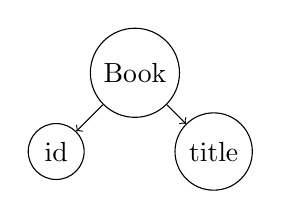
\begin{tikzpicture}
            \node[circle, draw] (n1) at (1,1) {Book};
            \node[circle, draw] (n2) at (0,0) {id};
            \node[circle, draw] (n3) at (2,0) {title};
            \draw[->] (n1) -- (n2);
            \draw[->] (n1) -- (n3);
        \end{tikzpicture}
    \end{minipage}
\end{figure}

Dann hat der Typ $Buch$ zwei Kanten, zu den jeweils beiden definierten Feldern $id$ und $title$.
In Kapitel~\ref{schematypes} haben wir festegelegt, dass Skalare Typen keine eigenen Beziehungen haben.
Daher können die Felder $id$ und $title$ selbst keine ausgehenden Kanten haben.
Das generelle Prinzip der Graphbildung ist:

\begin{enumerate}
    \item Erstelle Knoten aus jedem Typen und den definierten Feldern des Knotens
    \item Ziehe für jeden Typ seine Kanten, indem alle Felder des Typens zum entsprechenden Knoten verbunden werden
\end{enumerate}

Nach diesem Prinzip kann nun aus einem beliebig großen Schema ein gerichteter Graph gebildet werden.
\newpage

\subsection{Abfragen im Graphen}
\label{abfrgraph}

Wie behandelt GraphQL nun Anfragen intern und wie können wir dies in unserer Graphstruktur visualisieren?
Für die Erklärung definieren wir zuerst ein Schema als Beispiel:

\begin{figure}[htb]
    \centering
    \begin{minipage}[h!tb]{0.4\textwidth}
        \begin{lstlisting}[language=GraphQL]
type Query {
    buch: Buch
    autor: Autor
}
type Buch {
    id: Int
    title: String
    autor: Autor
    verleger: Verlag
}
        \end{lstlisting}
    \end{minipage}
    \hfill
    \begin{minipage}[h!tb]{0.4\textwidth}
        \begin{lstlisting}[language=GraphQL]
type Author {
    id: Int
    name: String
    schrieb: [Buch!]
}
type Verlag {
    name: String
}
        \end{lstlisting}
    \end{minipage}
    \label{schemdef}
    \caption{Schemadefinition}
\end{figure}

Dieses Schema wird durch folgenden Graphen repräsentiert: \\

\begin{figure}[htb]
    \centering
    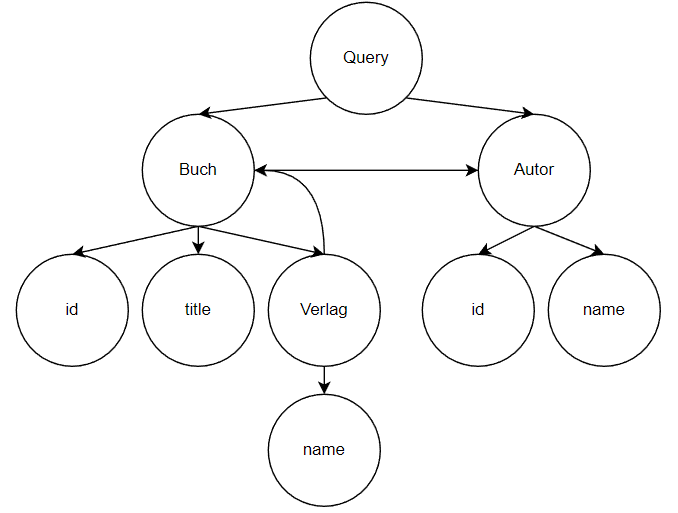
\includegraphics[width=\textwidth,height=0.4\textheight,keepaspectratio]{img/graph}
    \caption{Graph für Schemadefinition aus Abbildung~\ref{schemdef}}
    \label{schemg}
\end{figure}

Valide Anfragen an eine GraphQL-API sind nun alle Pfade, die mit Startknoten $Query$ beginnen und mindestens einen Knoten beinhalten,
der keine ausgehenden Kanten hat (also ein Scalar-Type)~\cite[vgl. Modelling with GraphQL]{graphqlgraphtheory}.
Auf jeder Ebene des Graphens werden Resolver ausgeführt welche für die Datenbereitstellung verantwortlich sind.
Wollen wir nun einen GraphQL-Server mit dem zuvor definierten Schema ein Buch mit id, Titel und Verlag mit Verlagsnamen abfragen,
so können wir diese Query nutzen: \verb+{ buch { id title verleger { name }}}+.

\begin{figure}[htb]
    \centering
    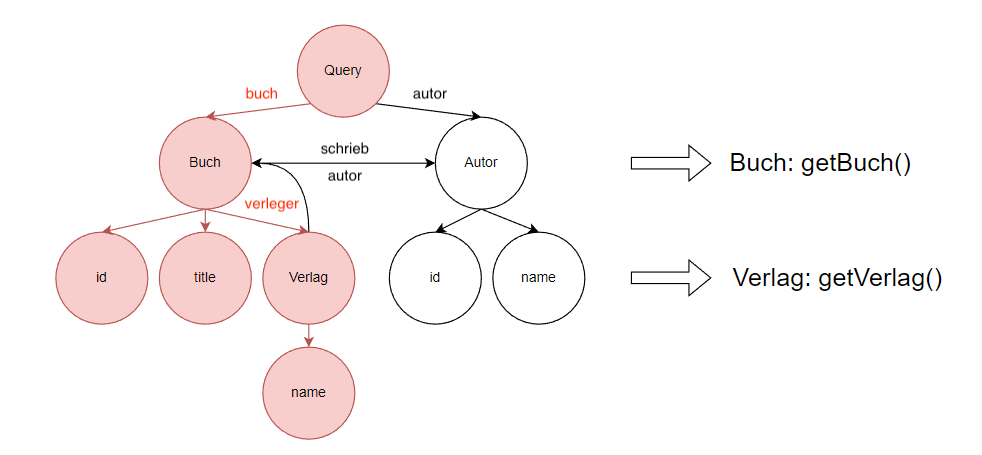
\includegraphics[width=\textwidth,height=0.4\textheight,keepaspectratio]{img/graphresolver}
    \caption{Graph für Abfrage nach~\cite{graphqlgraphtheory}}
    \label{abfrage}
\end{figure}

Mit Ausführung dieser Query wird initial der Resolver $getBuch()$ ausgeführt.
Liefert dieser ein valides Ergebnis zurück, also gibt es ein solches Buch,
dann wird der nächste Resolver $getVerlag()$ ausgeführt~\cite[vgl. Resolver]{graphqlgraphtheory}.
Dadurch, dass die Typen $Buch$ und $Autor$ aufeinander verweisen, ist der Graph des Schemas zyklisch und die Pfadmenge,
das heißt die validen Abfragen die gestellt werden können, unendlich.
